\documentclass[11pt]{beamer}
\usepackage[utf8]{inputenc}
\usepackage[T1]{fontenc}
\usepackage{lmodern}

\usepackage{amsmath,amssymb}
\usepackage[shortlabels]{enumitem}
\usepackage{graphicx}
\usepackage{algorithm}
\usepackage{algpseudocode}

\title{Quasi-random number generator}
\author[Ines Meršak]{Ines Meršak \\
    Mentor: doc.~dr.~Dejan Velušček}
\date{9.~6.~2017}

\usetheme{Madrid}
\usecolortheme{beaver}

\begin{document}
\begin{frame}
    \maketitle
\end{frame}

\begin{frame}{Pseudo-random vs.~quasi-random}
    \alert{Pseudo-random number} 
    \begin{itemize}
        \item computer-generated number
        \item appears to be random
        \item generated by an entirely deterministic process
    \end{itemize}

    \bigskip
    
    \bigskip
    
    \alert{Quasi-random number}
    \begin{itemize}
        \item low-discrepancy number
        \item taking previous draws into account
    \end{itemize}
\end{frame}

\begin{frame}
    \begin{figure}
        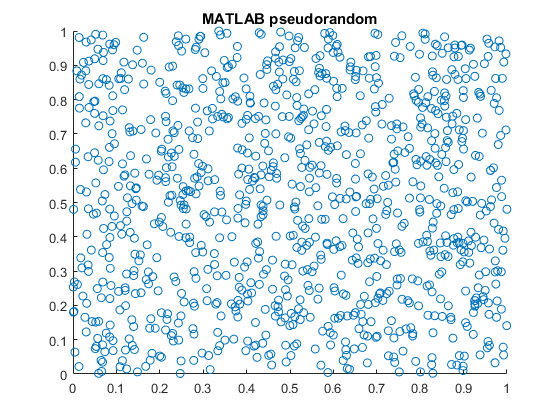
\includegraphics[width=170pt]{matlab-pseudorandom-points.png}
        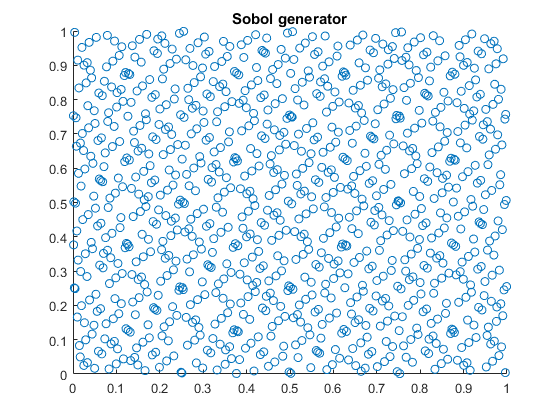
\includegraphics[width=170pt]{sobol-points.png}
    \caption{The comparison between pseudo- (left) and quasi-random numbers.}
    \end{figure}
\end{frame}

\begin{frame}{Usage}
    \begin{itemize}[--]
        \item useful in computational problems
        \medskip
        \item popular for financial Monte Carlo calculations 
        \medskip
        \item asymptotic convergence is faster than when using pseudo-random numbers

    \end{itemize}
\end{frame}

\begin{frame}{Sobol' numbers}
    \begin{algorithm}[H]
        \caption{Generates the $d$-dimensional vector $x_n$ in the Sobol sequence.}\label{alg:alg1}
        \begin{algorithmic}[1]
            \State $\gamma(n) = n$ or $\gamma(n) = G(n)$
            \For{$k = 1, \ldots, d$}
            \State $p_k(z) = a_{k0} z^{g_k} + a_{k1} z^{g_k-1} + \ldots + a_{k (g_k-1)} z + a_{k g_k}$
            \State calculate the direction integers $v_{kl}$ using $a_{kj}$ and binary addition
            \State calculate $x_{nk}$ based on which bits in $\gamma(n)$ are set
            \EndFor
        \end{algorithmic}
        \label{alg_1}
    \end{algorithm}
\end{frame}

\begin{frame}{Gray code}
    \begin{itemize}[--]
        \item any unique representation of $n$ can be used for $\gamma(n)$
        \medskip
        
        \item $G(n)$ switches only one single bit for every increment in $n$
        \medskip
        
        \item this means that a single XOR operation has to be carried out for each dimension: 
    \end{itemize}
    \[ x_{nk} = x_{(n-1)k} \oplus v_{kj} \]

\end{frame}

\begin{frame}{Gray code vs.~not Gray code}
    \begin{figure}
        \centering
        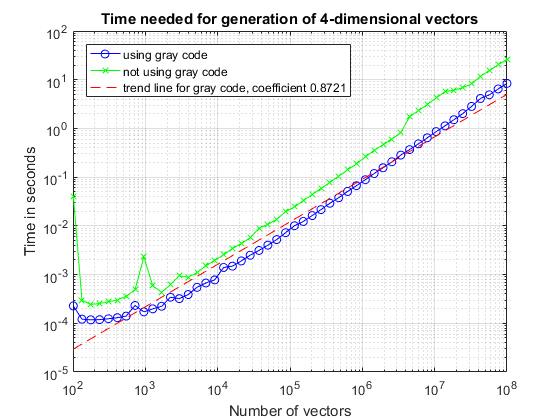
\includegraphics[width=260pt]{time.png}
    \end{figure}
\end{frame}

\begin{frame}{Monte Carlo integration}
    \begin{figure}
        \centering
        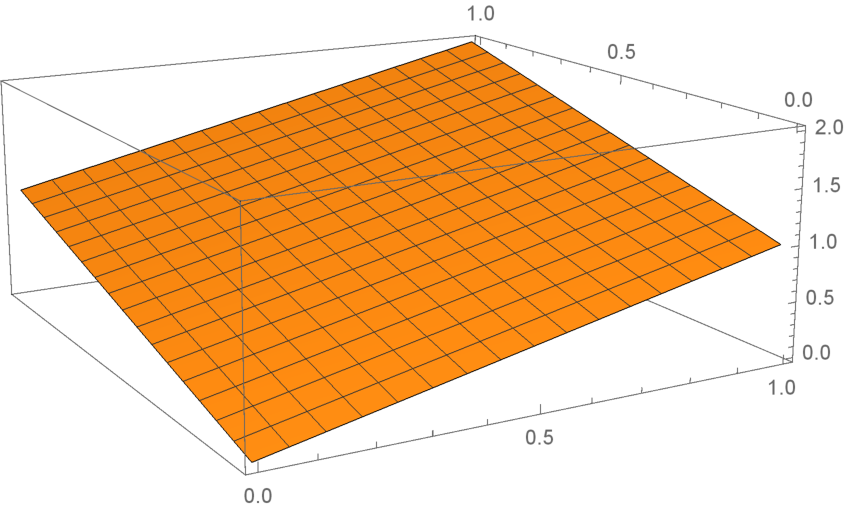
\includegraphics[width=250pt]{monte-carlo-xplusy.pdf}
        \caption{Plot of function $x+y$.}
    \end{figure}
\end{frame}

\begin{frame}
    \begin{figure}
        \centering
        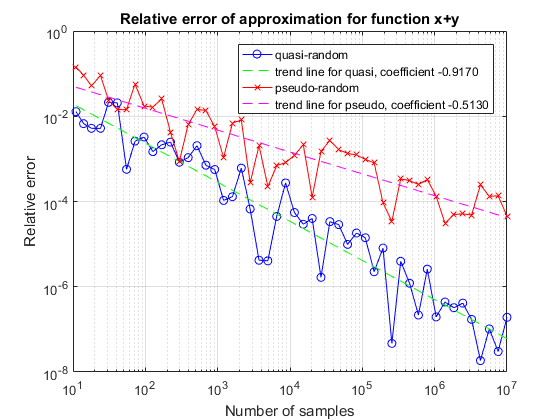
\includegraphics[width=250pt]{monte-carlo-xplusy-error.png}
    \end{figure}
\end{frame}

\begin{frame}
    \begin{figure}
        \centering
        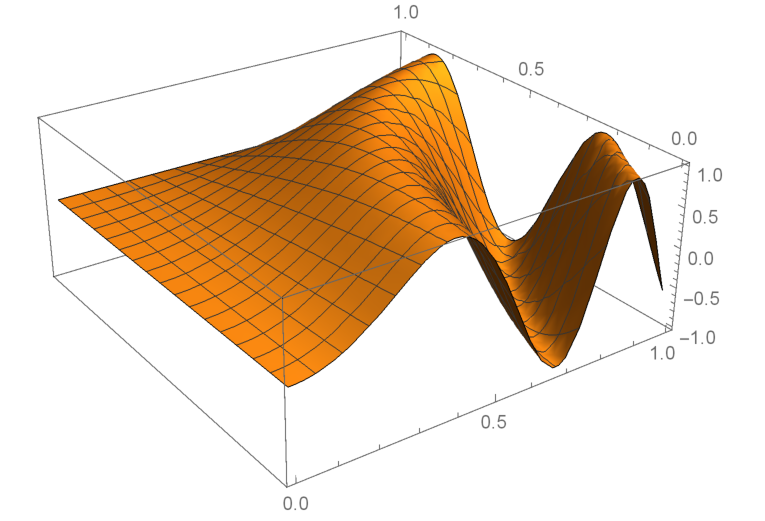
\includegraphics[width=250pt]{monte-carlo-sin.pdf}
        \caption{Plot of function $\sin(10 x^2 (1-y))$.}
    \end{figure}
\end{frame}

\begin{frame}
    \begin{figure}
        \centering
        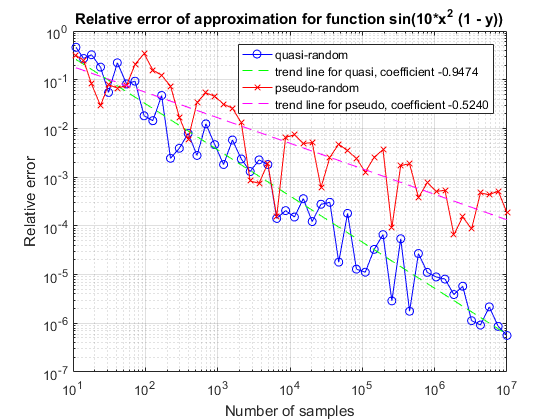
\includegraphics[width=250pt]{monte-carlo-sin-error.png}
    \end{figure}
\end{frame}

\end{document}